% !Mode:: "TeX:UTF-8"
% !TEX root = main.tex
% !TeX spellcheck = en_US

\documentclass{article}
% \documentclass[fontset=none]{ctexart}

\usepackage{seqsplit}
\usepackage{xparse}  % 用于定义新的命令
\usepackage{expl3}  % LaTeX3 编程接口
\usepackage{iftex}
\usepackage[T1]{fontenc}

% ---------------------------------------------------------------------------- %
%                                  polyglossia                                 %
% ---------------------------------------------------------------------------- %
\ifLuaTeX
% LuaTeX使用TH-Times字体必须开启polyglossia;XeTeX+CTeX使用pmhanguljamo需开启polyglossia
\usepackage{polyglossia}
\setmainlanguage{english}
% \newfontfamily\cjkfont{Noto Sans CJK SC}
\setotherlanguage{korean}
% \setotherlanguage{marshallese}
% \setotherlanguage{phagspa}
% ---------------------------- polyglossia参数控制图标题注 --------------------------- %
\gappto\captionsenglish{\def\tablename{表}}
\gappto\captionsenglish{\def\figurename{图}}
\gappto\captionsenglish{\def\contentsname{目~~录}}
\gappto\captionsenglish{\def\listfigurename{图~~片}}
\gappto\captionsenglish{\def\listtablename{表~~格}}
\fi

\usepackage{fontspec}
\usepackage{xunicode-addon}
\usepackage[UTF8,zihao=-4]{ctex}
\ctexset{
  figurename = 图,
  tablename  = 表,
  contentsname = {目~~录}
}%
\let\kaiti=\kaishu
% \ctexset{
%     fontset=windows
% }

% ------------------------------ caption宏包控制图标题注 ----------------------------- %
% \usepackage{caption}
% \captionsetup[figure]{name=图}
% \captionsetup[table]{name=表}
\renewcommand{\thetable}{\thesection-\arabic{table}}
\renewcommand{\thefigure}{\thesection-\arabic{figure}}


% ---------------------------------- 标题格式设置 ---------------------------------- %
\usepackage{titleref}
\usepackage{titlesec}
%\titlespacing*{hcommandi}{hlefti}{hbefore-sepi}{hafter-sepi}[hright-sepi]
\titlespacing*{\section}{0pt}{\baselineskip}{0.5\baselineskip}
\titlespacing*{\subsection}{0pt}{0.5\baselineskip}{0.5\baselineskip}
\titlespacing*{\subsubsection}{0pt}{0.5\baselineskip}{0pt}
\titlespacing{\paragraph}{2em}{0.5\baselineskip}{1em}
% 这里利用titleformat*简单做设置,也可以利用titleformat做详细设置
% \titleformat*{\section}{\zihao{-3}\bfseries\heiti}
% \titleformat*{\subsection}{\zihao{4}\bfseries\heiti}
\titleformat*{\subsubsection}{\zihao{-4}\bfseries\kaiti}
% \renewcommand{\contentsname}{\zihao{4}目~~录}



\usepackage{xurl}
\usepackage{listings}
\usepackage{makecell}


% ---------------------------------------------------------------------------- %
%                                     西文字体                                  %
% ---------------------------------------------------------------------------- %
% 天珩字库 TH-Times TrueType TTC http://cheonhyeong.com/Tools/Times.html st ct Qu 2nd 等默认皆连字
% \setmainfont{TH-Times}[AutoFakeBold]
\setmainfont{texgyrepagella}[
% \setmainfont{texgyretermes}[      %仿TimesNewRoman字体
  Extension      = .otf,
  UprightFont    = *-regular,
  BoldFont       = *-bold,
  ItalicFont     = *-italic,
  BoldItalicFont = *-bolditalic,
  Ligatures      = TeX,
]%
\setsansfont{texgyreheros}[
  Extension      = .otf,
  UprightFont    = *-regular,
  BoldFont       = *-bold,
  ItalicFont     = *-italic,
  BoldItalicFont = *-bolditalic,
]%
% \setmonofont{texgyrecursor}[
%   Extension      = .otf,
%   UprightFont    = *-regular,
%   BoldFont       = *-bold,
%   ItalicFont     = *-italic,
%   BoldItalicFont = *-bolditalic,
%   Scale          = MatchLowercase,
%   Ligatures      = CommonOff,
% ]%

%手动fallback用TH-Times
\newfontfamily\fb{TH-Times}
\newfontfamily\fbtk{TH-Times}[Language=Turkish]
\newfontfamily\fbcn{TH-Times}[Language={Chinese Simplified}]
\newfontfamily\fbtw{TH-Times}[Language={Chinese Traditional}]
\newfontfamily\fbjp{TH-Times}[Language={Japanese}]
\newCJKfontfamily\cjkcn{Noto Serif CJK SC}[Language={Chinese Simplified}]
\newCJKfontfamily\cjktw{Noto Serif CJK TC}[Language={Chinese Traditional}]
\newCJKfontfamily\fbpunctw{TH-Times}[Language={Chinese Traditional}] % for demo
\newfontfamily\hangulfont{Noto Serif CJK KR}[Script=Hangul]%
% \newfontfamily\phagspafont{TH-Times}[Script=Phags-pa]%
\newfontfamily\mongolianfont{TH-Times}[Script=Mongolian]%
% \newfontfamily\marshallesefont{TH-Times}% for demo
% ----------------------------------- 八思巴文 ----------------------------------- %
% 处理连字(IUEO的位置变体)需换用字体支持Script=Phags-pa
% \newfontfamily\psp{Noto Sans PhagsPa}[Script=Phags-pa] %Linux下NotoSansPhagsPa
% \newfontfamily\psp{Microsoft PhagsPa}[Script=Phags-pa] %Windows下Microsoft PhagsPa
\newfontfamily\psp{TH-Times}[Script=Phags-pa] %TH-Times修正了NotoSansPhagsPa的错误

%----------------------------------------------------------------------------------
%%CJK配置
\ifXeTeX
\xeCJKDeclareCharClass{CJK}{%带圈数字划给CJK
  "24EA,        % ⓪
  "2460->"2473, % ①->⑳
  "3251->"32BF, % ㉑->㊿
  "24FF,        % ⓿
  "2776->"277F, % ❶->❿
  "24EB->"24F4  % ⓫->⓴
}

%定义CJK字体分区
\xeCJKDeclareSubCJKBlock{P0-CJKpart}{"2FF0->"2FFF, "3100->"312F, "31A0->"31BF, "31C0->"31EF} %第0平面部分CJK
% \xeCJKDeclareSubCJKBlock{CJKExtA}{"3400-> "4DBF} %CJK扩展A (思源宋体全收录)
% \xeCJKDeclareSubCJKBlock{CJKUnified}{"4E00 -> "9FFF} %CJK统一(思源宋体全收录)
% \xeCJKDeclareSubCJKBlock{CJKCompat}{"F900-> "FAFF} %CJK兼容(思源宋体收录不全)
\xeCJKDeclareSubCJKBlock{CJKCompat-Source}{"FA6E-> "FAFF} %CJK兼容,思源宋体不支持的部分
% \xeCJKDeclareSubCJKBlock{SPUA}{ "E400 -> "E4DA , "E500 -> "E5E8 , "E600 -> "E6CE } %私用区
\xeCJKDeclareSubCJKBlock{P2}{ "20000 -> "2EE5F } %第2平面汉字(CJK扩展BCDEFI)
\xeCJKDeclareSubCJKBlock{P3}{ "30000 -> "323AF } %第3平面汉字(CJK扩展GH)
% \xeCJKDeclareSubCJKBlock{P16}{ "100000 -> "10FFFF } %第16平面汉字(补充私用区B)
% \xeCJKDeclareSubCJKBlock{Jamo}{ "1100->"11FF, "3130->"318F, "A960->"A97F, "D7B0->"D7FF} %谚文字母

\xeCJKsetup{
    AutoFallBack
}
\newCJKfontfamily\oldjamo{Noto Serif CJK KR}[Script=Hangul] %旧谚文

%设置中文字体
\setCJKmainfont[
    CJKCompat-Source=TH-Tshyn-P0,  % 思源宋体CJK兼容区缺失的,
    P0-CJKpart=TH-Tshyn-P0,            % 0平面部分字,
    P2=TH-Tshyn-P2,                % 2平面,
    P3=TH-Tshyn-P1,                % 3平面字交给 天珩字库 http://cheonhyeong.com/Simplified/download.html
    BoldFont={Noto Sans CJK SC},
    ItalicFont={AR PL KaitiM GB}, % TeX楷体
    % ]{Source Han Serif SC} %思源宋体
    ]{Noto Serif CJK SC} %Noto CJK,缺字,扩展A不全、统一区不全

\setCJKfallbackfamilyfont{\CJKrmdefault} %CJKfallback字体列
    { 
      % {[Jamo,Script=Hangul]{Noto Serif CJK KR}},
      {TH-Times},{TH-Tshyn-P0},{TH-Tshyn-P2},{TH-Tshyn-P1}}

% \setCJKmonofont{Noto Sans CJK SC}

\XeTeXlinebreaklocale "zh"
\XeTeXlinebreakskip = 0pt plus 1pt
\xeCJKOffVerbAddon
\fi

\ifLuaTeX
%-----------------------------------------------------------------------------------
% 给圈码数字分区,糅合THUThesis与https://www.cnblogs.com/coderzjz/p/15821966.html
% ctex 将带圈数字 U+2460–U+24FF 归入字符范围 3(ALchar),这里改回范围 6(JAchar)
\ltjdefcharrange{6}{%
%带圈字母数字,CJK汉字部首补充,【修改】CJK符号和标点,汉文训读符号,片假名语音扩展
"2460-"24FF, "2E80-"2EFF, "3000-"303F, "3190-"319F, "31F0-"4DBF,
%CJK统一,CJK兼容,竖排形式,CJK兼容形式(竖排标点),半角及全角字符
"4E00-"9FFF, "F900-"FAFF, "FE10-"FE1F, "FE30-"FE6F, "FF00-"FFEF,
%假名补充 假名扩展A 小型假名扩展,带圈字母数字补充 带圈表意文字补充,CJK二三平面,变体选择符补充
"1B000-"1B16F, "1F100-"1F2FF, "20000-"3FFFF, "E0100-"E01EF,
%【新增】圈1-10反白,CJK扩展A,注音符号,注音扩展
"2776-"277F, "3400-"4DBF, "3100-"312F, "31A0-"31BF,"1100-"11FF,"3130-"318F,"A960-"A97F}
% ------------------------------------ 谚文 ------------------------------------ %
\ltjdefcharrange{3}{
  "1100-"11FF,"3130-"318F,"A960-"A97F,"D7B0-"D7FF,"302E-"302F %谚文声调附点 302E 302F
}
\ltjdefcharrange{3}{
  "AC00-"D7AF % 现代韩语音节,开启后ctex+polyglossia可谚文傍点,但正文CJK字体无法显示韩语
}
%-----------------------------------------------------------------------------------
\ctexset
{
    declarecharrange =
        {
            {P0-CJKpart} {"2FF0 -> "2FFF , "3100 -> "312F , "31A0 -> "31BF , "31C0 -> "31EF} , %P0的部分CJK
            {CJKCompat-Source} {"FA6E-> "FAFF}, %CJK兼容 思源宋体不支持的部分
            {P2} { "20000 -> "2EE5F } , %第2平面汉字
            {P3} { "30000 -> "323AF } , %第3平面汉字
            % {jamo} {"1100->"11FF,"3130->"318F,"A960->"A97F,"D7B0->"D7FF} , %谚文字母 谚文兼容字母 扩展A 扩展B
        }
}
\newfontfamily\oldjamo{Noto Serif CJK KR}[Script=Hangul]
% \newCJKfontfamily\oldCJKjamo{Noto Serif CJK KR}[Script=Hangul]


%设置中文字体
% \setCJKmainfont{Noto Serif CJK SC}
\setCJKmainfont{Source Han Serif SC} %用下载的思源宋体,而非debian源里的思源宋体,支持的字更多
[
    BoldFont={Noto Sans CJK SC},
    % ItalicFont={KaiTi},
    ItalicFont={AR PL KaitiM GB}, % TeX楷体
    Script=CJK,                
    AlternateFont={
        % {jamo} {Noto Serif CJK KR} {Script=Hangul},
        {P0-CJKpart,CJKCompat-Source} {TH-Tshyn-P0}, 
        {P2} {TH-Tshyn-P2}, 
        {P3} {TH-Tshyn-P1}, % 天珩字库 http://cheonhyeong.com/Simplified/download.html
    }
] %思源宋体
% \setCJKmainfont[CharRange={jamo},Script=Hangul]{Noto Serif CJK KR}
% \usepackage[hangul]{luatexko} %LuaTeX下利用luatexko宏包正确显示谚文(要放在ctex之后,否则会冲突,无必要先别开。会有代价吗?已知行距会增大。)
\fi

% ----------------------------- 重定义\songti \heiti ---------------------------- %
\setCJKfamilyfont{zhsong}{Source Han Serif SC}
[
    UprightFont = *-Regular,
    BoldFont = *-Bold,
    ItalicFont = *-Regular,
    BoldItalicFont = *-Bold
]
\setCJKfamilyfont{zhhei}{Noto Sans CJK SC}
[
    UprightFont = *-Regular,
    BoldFont = *-Bold,
    ItalicFont = *-Regular,
    BoldItalicFont = *-Bold
]
% ---------------------------------------------------------------------------- %

\usepackage[pmfont={Noto Serif CJK KR}]{pmhanguljamo}

%------------------------------------------------------------------------------------
%% 带圈数字 https://stone-zeng.site/2019-02-09-circled-numbers
% 【注意!】:fontspec,xunicode-addon要置于ctex之前
% XeLaTeX 下需要把全体带圈数字都设置成 Default 类(上方有CJK了,不需要)
% \xeCJKDeclareCharClass{Default}{"24EA, "2460->"2473, "3251->"32BF}
% 将中文字体声明为(西文)字体族(我这思源宋缩放时会有字重问题,TH-Times会好些)
% \newfontfamily\EnclosedNumbers{TH-Times} %天珩字库
\newfontfamily\EnclosedNumbers{Noto Serif CJK SC}
% 放置钩子,只让带圈字符才需更换字体
\AtBeginUTFCommand[\textcircled]{\begingroup\EnclosedNumbers}
\AtEndUTFCommand[\textcircled]{\endgroup}
%-------------------------------------------------------------------------------------


% ------------------------------------ 删除线 ----------------------------------- %
\ifLuaTeX
  \usepackage{luacolor}
  \usepackage[soul]{lua-ul} %eisvogel模板所采用,配合markdown删除线
  \newcommand*{\sout}[1]{\st{#1}}
  % \usepackage{soul}
  % \usepackage{ulem} %不支持中文
\fi
\ifXeTeX
  \usepackage{xeCJKfntef}
  % \renewcommand{\st}[1]{\sout{#1}}
\fi


\usepackage[paperwidth=210mm,paperheight=290mm,left=25mm,right=25mm,top=25mm, bottom=20mm,showcrop]{geometry}

% \PassOptionsToPackage{hyphens}{url}\usepackage{hyperref}
\makeatletter
\g@addto@macro\UrlBreaks{%
  \do0\do1\do2\do3\do4\do5\do6\do7\do8\do9%
  \do\A\do\B\do\C\do\D\do\E\do\F\do\G\do\H\do\I\do\J\do\K\do\L\do\M
  \do\N\do\O\do\P\do\Q\do\R\do\S\do\T\do\U\do\V\do\W\do\X\do\Y\do\Z
  \do\a\do\b\do\c\do\d\do\e\do\f\do\g\do\h\do\i\do\j\do\k\do\l\do\m
  \do\n\do\o\do\p\do\q\do\r\do\s\do\t\do\u\do\v\do\w\do\x\do\y\do\z
}
\Urlmuskip=0mu plus 0.1mu
\makeatother
% \urlstyle{rm}
\urlstyle{same}
% 替换\url为支持cjk的衬线字体
% \newfontfamily\urlfontcjk{Noto Serif CJK SC}%用于支持url的字体(待删)
% \def\UrlFont{\urlfontcjk}


\usepackage{footmisc}

\usepackage{metalogo}
\usepackage{cprotect}
\usepackage{hyperref}
\hypersetup{
    CJKbookmarks,
    breaklinks,
}

\begin{document}

\title{ \Huge \LaTeX 字体测试\\ \vspace*{0.5em}
\large 本次使用
\ifLuaTeX
\LuaLaTeX 
\fi
\ifXeTeX
\XeLaTeX 
\fi
编译}
\author{moonhikari}
\date{2024/8/30}
\maketitle

\tableofcontents \newpage

% !Mode:: "TeX:UTF-8"
% !TEX root = ../main.tex

\section{Test Fonts 测试字体}

\subsection{字体集 Fontset}

\subsubsection{小标题 Heading3}

自动字体:普通,\verb|\textbf| \textbf{粗体},\verb|\textit| \textit{意大利斜体},\verb|\textsl| \textsl{倾斜体}

单独字体:{\songti 宋体},{\heiti 黑体},{\kaiti 楷体}
,{\fangsong 仿宋}% Ubuntu没有仿宋
% ,{\lishu 隶书},{\youyuan 幼圆}, % windows、founder和macnew中有隶书、幼圆
% ,{\yahei 微软雅黑} % windows中另有微软雅黑
% ,{\pingfang 苹方} % macnew另有苹方

Pandoc转义字体:\textbf{粗体},\verb|\emph| \emph{斜体},\verb|\sout| \sout{删除线}

English Text, \textbf{Bold English Text}, \textit{Italic English Text}

\subsection{带圈数字}

Unicode:
⓪ ① ② ③ ④ ⑤ ⑥ ⑦ ⑧ ⑨ ⑩ ⑪	⑫ ⑬	⑭ ⑮	⑯ ⑰ ⑱ ⑲	⑳ ㉑ ㉒	㉓ ㉔ ㉕ ㉖ ㉗ ㉘ ㉙ ㉚ ㉛ ㉜ ㉝ ㉞	㉟ ㊱ ㊲ ㊳ ㊴ ㊵ ㊶ ㊷ ㊸ ㊹ ㊺	㊻ ㊼ ㊽ ㊾ ㊿ 

\verb|\textcirciled{}|:
\textcircled{5} \textcircled{10} \textcircled{19} \textcircled{20} \textcircled{25} , \textcircled{56} \textcircled{87}  \textcircled{190}

圈码在正文中(检测基线平齐):

⑲ 榷盐院是官府垄断食盐产销的专门机构。其通常做法,是向盐户牧盐(即民制官收),再将盐税加入卖价,售予商人,听其运销,所过州县不再征税\footnote{宝坻县志编修委员会. 宝坻县志. 第一编, 建置区划, 置县. 天津社会科学院出版社. 1995-05, 第89页.};

⑳ 燕云一十六州:即幽、蓟、瀛、莫、涿、檀、顺、新、妫、儒、武、云、应、寰、朔、蔚州,相当于以今北京和大同为中心,东至河北遵化,北迄长城,西界山西神池,南至天津、河间、保定及山西繁峙、宁武一线以北地区\footnote{宝坻县志编修委员会. 宝坻县志. 第一编, 建置区划, 置县. 天津社会科学院出版社. 1995-05, 第89页.};

% \subsection{TH-Times\footnote{见\url{http://cheonhyeong.com/Tools/Times.html}}特色}
\subsection[TH-Times特色]{TH-Times{\protect\footnote{见\url{http://cheonhyeong.com/Tools/Times.html}}}特色}
音标:{\fb tʃi˥˧/ʈʂɨ˥˧ },西文 {\fb Бао-ди},


零宽附标 {\fb j+ü᪻̄=jū},环绕附标 {\fb Щ⃣ ​}

\subsubsection*{语言本地化:}

英语 {\fb rahîm M̧ajeļ gá}
, 土耳其语
% \begin{selectlanguage}{turkish}
    {\fbtk rahîm M̧ajeļ gá}
% \end{selectlanguage}
, 马绍尔语不适配
% \begin{selectlanguage}{marshallese}
    {rahîm M̧ajeļ gá}
% \end{selectlanguage}
, 简体中文
% \begin{selectlanguage}{chinese}
    {\fbcn rahîm M̧ajeļ gá}
% \end{selectlanguage}

简体中文{\fbcn 🀆 🀐 🩠 🩩},日本{\fbjp 🀆 🀐 🩠 🩩}

TH-Times定义为CJK字体:简体中文~文字{\fbcn ,}文字{\fbcn 、}\; 台湾繁体~{\cjktw 文字}{\fbpunctw ,}{\cjktw 文字}{\fbpunctw 、}

直接用NotoCJK对应字体:简体中文~{\cjkcn 文字,文字、}\; 台湾繁体~{\cjktw 文字,文字、}

\subsection{测试连字}

\noindent main字体:

\begin{quote}
    AE ae OE oe ff fi fl ij st ft et fs ffi ffl fa fe fo fr fb fh fu fy ch ct Qu Th mistake 2nd
\end{quote}


\noindent TH-Times字体:

\begin{quote}
    {\fb AE ae OE oe ff fi fl ij st ft et fs ffi ffl fa fe fo fr fb fh fu fy ch ct Qu Th mistake 2nd 2th 12th 12nd física Schiff‌fahrt Schieſ‍splat‍z}
\end{quote}


\noindent 插入ZWNJ \verb|\char"200C{}| 以停止连字:

\begin{quote}
    {\fb A\char"200C{}E a\char"200Ce O\char"200C{}E o\char"200Ce f\char"200Cf f\char"200Ci f\char"200Cl i\char"200Cj s\char"200Ct f\char"200Ct e\char"200Ct f\char"200Cs f\char"200Cf\char"200Ci f\char"200Cf\char"200Cl f\char"200Ca f\char"200Ce f\char"200Co f\char"200Cr f\char"200Cb f\char"200Ch f\char"200Cu f\char"200Cy c\char"200Ch c\char"200Ct Q\char"200Cu T\char"200Ch mis\char"200Ctake 2\char"200Cnd}
\end{quote}


\noindent 五度标记法连字 {\fb ˥˩˨˦˧˥˩˨˦˧˥˩˨˦˧, ꜔꜓꜕꜖꜒꜔꜓꜕꜖꜒꜔꜓꜕꜖꜒}

\subsection{变体字符}


蒙古文同一字母存在独立、字首、字中、字尾形式的不同变体,使用自由变体选择符(FVS,\verb|"180B、"180C、"180D|)实现。
八思巴文(1269年~1368年)有6个字母存在反转形式变体,使用标准变体序列(SVS,VS01 \verb|"FE00|)实现,以上见表\ref{tab:svs}。另八思巴文有4个元音存在位置变体,由字体引擎处理,见表\ref{tab:my_label}。


\begin{table}[!ht]
    \caption{Mongolian variants tests}
    \centering
    \begin{tabular}{llll}
    \hline
        预期字形 & 显示 & 变形类型 & 测试内容 \\ \hline
        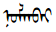
\includegraphics[height=1em]{figures/nomlabai.png} & \mongolianfont{ᠨᠣᠮ‍ᠯᠠᠪᠠᠢ} & 非强制 & 带有ZWJ的历史连字  \\ 
        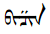
\includegraphics[height=1em]{figures/bischin.png} & \mongolianfont{ᠪᠢᡸᠢᠨ} & 强制 & U+1878能否为变形引擎所支持  \\ 
        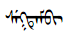
\includegraphics[height=1em]{figures/sektembi.png} & \mongolianfont{ᠰᡝᡴ᠏ᡨᡝᠮᠪᡳ} & 强制 & U+180F能否为变形引擎所支持  \\ 
        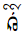
\includegraphics[height=1em]{figures/go.png} & \mongolianfont{ᡬᢅᠣ} & 强制 & baluda附标归位  \\ 
        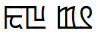
\includegraphics[height=1em]{figures/ttatthi.png} & \psp{ꡩꡖ︀ ꡪꡞ} & 强制 & 梵语镜像字母变形及SVS \\ \hline
    \end{tabular}
    \label{tab:svs}
\end{table}

\begin{table}[htbp]
    \caption{Test Phags-pa positional variants}
    \centering
    \begin{tabular}{rcccc}
        \hline
         & Isolate & Initial & Medial & Final\\
         \hline
        mainfont & ꡞ & ꡞꡄ & ꡄꡞꡄ & ꡄꡞ\\
        TH-Times default & {\fb ꡞ} & {\fb ꡞꡄ} & {\fb ꡄꡞꡄ} & {\fb ꡄꡞ}\\
        \verb|Script=Phags-pa| font & {\psp ꡞ} & {\psp ꡞꡄ} & {\psp ꡄꡞꡄ} & {\psp ꡄꡞ}\\
        \hline
    \end{tabular}
    \label{tab:my_label}
\end{table}

彩色字体 {\fb TH-Fonts,🐱🐶 2️⃣ 🀄︎🀄️ 🀐󠁊󠁐󠁿 🩠󠁋󠁒󠁿 🩩󠁋󠁒󠁿 🀢 🩬 R☖,\par 🀔 + ZWJ(\verb|\char"200D|)+ 🟥 以显示红宝牌: 🀔\char"200D🟥 🀝‍🟥 🀋\char"200D🟥}

\subsection{CJK兼容区测试}

U+F90x	豈	更	車	賈	滑	串	句	龜	龜	契	金	喇	奈	懶	癩	羅

U+F91x	蘿	螺	裸	邏	樂	洛	烙	珞	落	酪	駱	亂	卵	欄	爛	蘭

U+F92x	鸞	嵐	濫	藍	襤	拉	臘	蠟	廊	朗	浪	狼	郎	來	冷	勞

U+F93x	擄	櫓	爐	盧	老	蘆	虜	路	露	魯	鷺	碌	祿	綠	菉	錄

U+F94x	鹿	論	壟	弄	籠	聾	牢	磊	賂	雷	壘	屢	樓	淚	漏	累

U+F95x	縷	陋	勒	肋	凜	凌	稜	綾	菱	陵	讀	拏	樂	諾	丹	寧

U+F96x	怒	率	異	北	磻	便	復	不	泌	數	索	參	塞	省	葉	說

U+F97x	殺	辰	沈	拾	若	掠	略	亮	兩	凉	梁	糧	良	諒	量	勵

U+F98x	呂	女	廬	旅	濾	礪	閭	驪	麗	黎	力	曆	歷	轢	年	憐

U+F99x	戀	撚	漣	煉	璉	秊	練	聯	輦	蓮	連	鍊	列	劣	咽	烈

U+F9Ax	裂	說	廉	念	捻	殮	簾	獵	令	囹	寧	嶺	怜	玲	瑩	羚

U+F9Bx	聆	鈴	零	靈	領	例	禮	醴	隸	惡	了	僚	寮	尿	料	樂

U+F9Cx	燎	療	蓼	遼	龍	暈	阮	劉	杻	柳	流	溜	琉	留	硫	紐

U+F9Dx	類	六	戮	陸	倫	崙	淪	輪	律	慄	栗	率	隆	利	吏	履

U+F9Ex	易	李	梨	泥	理	痢	罹	裏	裡	里	離	匿	溺	吝	燐	璘

U+F9Fx	藺	隣	鱗	麟	林	淋	臨	立	笠	粒	狀	炙	識	什	茶	刺

U+FA0x	切	度	拓	糖	宅	洞	暴	輻	行	降	見	廓	兀	嗀	﨎	﨏

U+FA1x	塚	﨑	晴	﨓	﨔	凞	猪	益	礼	神	祥	福	靖	精	羽	﨟

U+FA2x	蘒	﨡	諸	﨣	﨤	逸	都	﨧	﨨	﨩	飯	飼	館	鶴	郞	隷

U+FA3x	侮	僧	免	勉	勤	卑	喝	嘆	器	塀	墨	層	屮	悔	慨	憎

U+FA4x	懲	敏	既	暑	梅	海	渚	漢	煮	爫	琢	碑	社	祉	祈	祐

U+FA5x	祖	祝	禍	禎	穀	突	節	練	縉	繁	署	者	臭	艹	艹	著

U+FA6x	褐	視	謁	謹	賓	贈	辶	逸	難	響	頻	恵	𤋮	舘		

U+FA7x	並	况	全	侀	充	冀	勇	勺	喝	啕	喙	嗢	塚	墳	奄	奔

U+FA8x	婢	嬨	廒	廙	彩	徭	惘	慎	愈	憎	慠	懲	戴	揄	搜	摒

U+FA9x	敖	晴	朗	望	杖	歹	殺	流	滛	滋	漢	瀞	煮	瞧	爵	犯

U+FAAx	猪	瑱	甆	画	瘝	瘟	益	盛	直	睊	着	磌	窱	節	类	絛

U+FABx	練	缾	者	荒	華	蝹	襁	覆	視	調	諸	請	謁	諾	諭	謹

U+FACx	變	贈	輸	遲	醙	鉶	陼	難	靖	韛	響	頋	頻	鬒	龜	𢡊

U+FADx	𢡄	𣏕	㮝	䀘	䀹	𥉉	𥳐	𧻓	齃	龎

\newpage
% !Mode:: "TeX:UTF-8"
% !TEX root = ../main.tex

\section{Test Unicode}

八思巴字(A840-A877):

{\psp ꡀꡁꡂꡃꡄꡅꡆꡇꡈꡉꡊꡋꡌꡍꡎꡏꡐꡑꡒꡓꡔꡕꡖꡗꡘ

ꡙꡚꡛꡜꡝꡞꡟꡠꡡꡢꡣꡤꡥꡦꡧꡨꡩꡪꡫꡬꡭꡮꡯꡰꡱꡲꡳ꡴꡵꡶꡷}


注音符号(3100-312F):\*ㄅㄆㄇㄈㄉㄊㄋㄌㄍㄎㄏㄐㄑㄒㄓㄔㄕㄖㄗㄘㄙㄚㄛㄜㄝㄞㄟㄠㄡㄢㄣㄤㄥㄦㄧㄨㄩㄪㄫㄬㄭㄮㄯ

注音扩展(31A0-31BF):ㆠㆡㆢㆣㆤㆥㆦㆧㆨㆩㆪㆫㆬㆭㆮㆯㆰㆱㆲㆳㆴㆵㆶㆷㆸㆹㆺㆻㆼㆽㆾㆿ

CJK笔画(31C0-31EF):㇀㇁㇂㇃㇄㇅㇆㇇㇈㇉㇊㇋㇌㇍㇎㇏㇐㇑㇒㇓㇔㇕㇖㇗㇘㇙㇚㇛㇜㇝㇞㇟㇠㇡㇢㇣——㇯

CJK扩展A(3400-4DBF):㐀㐁㐂㐃㐄㐅㐆㐇㐈㐉㐊㐋㐌㐍㐎㐏——䶰䶱䶲䶳䶴䶵䶶䶷䶸䶹䶺䶻䶼䶽䶾䶿

CJK统一表意文字(4E00-9FFF):一丁丂七丄丅丆万丈三上下丌不与丏——鿰鿱鿲鿳鿴鿵鿶鿷鿸鿹鿺鿻鿼鿽鿾鿿

中日韩兼容表意文字(F900-FAFF):豈更車賈滑串句龜龜契金喇奈懶癩羅——𢡄𣏕㮝䀘䀹𥉉𥳐𧻓齃龎\*	

CJK扩展B(20000-2A6DF):𠀀𠀁𠀂𠀃𠀄𠀅𠀆𠀇𠀈𠀉𠀊𠀋𠀌𠀍𠀎𠀏——𪛐𪛑𪛒𪛓𪛔𪛕𪛖𪛗𪛘𪛙𪛚𪛛𪛜𪛝𪛞𪛟

CJK扩展C(2A700-2B73F):𪜀𪜁𪜂𪜃𪜄𪜅𪜆𪜇𪜈𪜉𪜊𪜋𪜌𪜍𪜎𪜏——𫜰𫜱𫜲𫜳𫜴𫜵𫜶𫜷𫜸𫜹\*

CJK扩展D(2B740-2B81F):𫝀𫝁𫝂𫝃𫝄𫝅𫝆𫝇𫝈𫝉𫝊𫝋𫝌𫝍𫝎𫝏——𫠐𫠑𫠒𫠓𫠔𫠕𫠖𫠗𫠘𫠙𫠚𫠛𫠜𫠝\*

CJK扩展E(2B820-2CEAF):𫠠𫠡𫠢𫠣𫠤𫠥𫠦𫠧𫠨𫠩𫠪𫠫𫠬𫠭𫠮𫠯——𬺐𬺑𬺒𬺓𬺔𬺕𬺖𬺗𬺘𬺙𬺚𬺛𬺜𬺝𬺞𬺟𬺠𬺡\*

CJK扩展F(2CEB0-2EBEF):𬺰𬺱𬺲𬺳𬺴𬺵𬺶𬺷𬺸𬺹𬺺𬺻𬺼𬺽𬺾𬺿——𮯐𮯑𮯒𮯓𮯔𮯕𮯖𮯗𮯘𮯙𮯚𮯛𮯜𮯝𮯞𮯟𮯠\*

CJK扩展I(2EBF0-2EE5F):𮯰𮯱𮯲𮯳𮯴𮯵𮯶𮯷𮯸𮯹𮯺𮯻𮯼𮯽𮯾𮯿——𮹐𮹑𮹒𮹓𮹔𮹕𮹖𮹗𮹘𮹙𮹚𮹛𮹜𮹝\*

CJK扩展G(30000-3134F):𰀀𰀁𰀂𰀃𰀄𰀅𰀆𰀇𰀈𰀉𰀊𰀋𰀌𰀍𰀎𰀏——𱍀𱍁𱍂𱍃𱍄𱍅𱍆𱍇𱍈𱍉𱍊\*

CJK扩展H(31350-323AF):𱍐𱍑𱍒𱍓𱍔𱍕𱍖𱍗𱍘𱍙𱍚𱍛𱍜𱍝𱍞𱍟——𲎠𲎡𲎢𲎣𲎤𲎥𲎦𲎧𲎨𲎩𲎪𲎫𲎬𲎭𲎮𲎯

谚文字母(Hangeul Jamo,1100-11FF):
{\oldjamo ᄀᄁᄂᄃᄄᄅᄆᄇᄈᄉᄊᄋᄌᄍᄎᄏ

——ᇰᇱᇲᇳᇴᇵᇶᇷᇸᇹᇺᇻᇼᇽᇾᇿ}

表意文字描述(IDC,2FF0-2FFF):⿰⿱⿲⿳⿴⿵⿶⿷⿸⿹⿺⿻⿼⿽⿾⿿

谚文兼容字母(Hangul Compatibility Jamo,3130-318F):\* 

{\oldjamo ㄱㄲㄳㄴㄵㄶㄷㄸㄹㄺㄻㄼㄽㄾㄿ——ㆀㆁㆂㆃㆄㆅㆆㆇㆈㆉㆊㆋㆌㆍㆎ }\*

谚文字母扩展A(A960-A97F):

{\oldjamo ꥠꥡꥢꥣꥤꥥꥦꥧꥨꥩꥪꥫꥬꥭꥮ
ꥰꥱꥲꥳꥴꥵꥶꥷꥸꥹꥺꥻꥼ}

谚文音节(AC00-D7AF):가각갂갃간갅갆갇갈갉갊갋갌갍갎갏——힠힡힢힣\*

谚文字母扩展B(D7B0-D7FF):

{\oldjamo ힰힱힲힳힴힵힶힷힸힹힺힻힼힽힾힿ——ퟰퟱퟲퟳퟴퟵퟶퟷퟸퟹퟺퟻ}

\subsection{Old Jamo}

旧谚文(另独立编码在私用区「汉阳PUA」E0BC-F8F7,此示例为字母拼成):

摘自\href{https://charset.fandom.com/ko/wiki/한양_PUA}{https://charset.fandom.com/ko/wiki/한양\_PUA}

{
    \oldjamo
F28 ᅎᆑ	ᅎᆑᆫ	ᅎᅳ	ᅎᅳᆫ	ᅎᅳᆺ	ᅎᅳᇫ	ᅎᅵ	ᅎᅵᆫ	ᅎᅵᆷ	ᅎᅵᇢ	ᅎᅵᇫ	ᅏᅡ	ᅏᅡᆫ	ᅏᅡᆷ	ᅏᅡᇢ	ᅏᅡᇰ

F29	ᅏᅢ	ᅏᅣ	ᅏᅣᆷ	ᅏᅣᇰ	ᅏᅥ	ᅏᅥᆫ	ᅏᅧ	ᅏᅧᆫ	ᅏᅨ	ᅏᅮ	ᅏᅱ	ᅏᅲ	ᅏᅲᇰ	ᅏᆑ	ᅏᆑᆫ	ᅏᅳ

F2A	ᅏᅳᇫ	ᅏᅳᇰ	ᅏᅵ	ᅏᅵᆫ	ᅏᆞ	ᅏᆡ	ᅐᅡ	ᅐᅡᆫ	ᅐᅡᆮ	ᅐᅡᆷ	ᅐᅡᇢ	ᅐᅡᆸ	ᅐᅢ	ᅐᅣ	ᅐᅣᆷ	ᅐᅣᇢ

F2B	ᅐᅣᇰ	ᅐᅧ	ᅐᅧᆫ	ᅐᅩ	ᅐᅪ	ᅐᅪᆼ	ᅐᅮ	ᅐᅮᆼ	ᅐᅮᇹ	ᅐᅲ	ᅐᅲᆨ	ᅐᅲᆫ	ᅐᅲᇰ	ᅐᆑ	ᅐᆑᆫ	ᅐᅳ

F2C	ᅐᅳᆷ	ᅐᅳᇫ	ᅐᅵ	ᅐᅵᆫ	ᅐᅵᇫ	ᅐᅵᇰ	ᅑᅡ	ᅑᅡᆫ	ᅑᅡᇂ	ᅑᅢ	ᅑᅣ	ᅑᅣᆷ	ᅑᅣᇢ	ᅑᅣᆸ	ᅑᅣᇰ	ᅑᅧ

F2D	ᅑᅧᆫ	ᅑᅮ	ᅑᅱ	ᅑᅲ	ᅑᅲᇰ	ᅑᆑ	ᅑᆑᆫ	ᅑᅳ	ᅑᅳᆷ	ᅑᅳᇢ	ᅑᅵ	ᅑᅵᆫ	ᅑᅵᆷ	ᅑᅵᇫ	ᅑᅵᇰ	차ᇙ

F2E	차ᇢ	차ᇦ	차ᇰ	차ᇹ	ᄎᅶ	챠ᇙ	챠ᇦ	챠ᇰ	챠ᇱ	ᄎᅸ	ᄎᅸᆯ	ᄎᆤ	처ᇫ	처ᇰ	ᄎᅼ	ᄎᅼᆫ

F2F	쳐ퟍ	쳐ퟎ	쳐ퟏ	쳐ᇙ	쳐ᇢ	쳐ᇰ	쳐ᇱ	쳐ᇹ	ᄎᅽ	ᄎᅾ	초ᇙ	초ᇢ	초ퟨ	초ᇫ	초ᇰ	촤ᇙ

F30	촤ᇰ	ᄎᆂ	쵸ᇢ	쵸ᇰ	ᄎᆇ	ᄎᆈ	ᄎᆈᆫ	추ᇙ	추ᇠ	추ᇢ	추ᇰ	추ᇹ	ᄎᆉ	ᄎᆉᆫ	ᄎᆉᆼ	ᄎᆊ

F31	춰ᇹ	ᄎힵ	ᄎᆌ	취ᇙ	취ᇹ	츄ᇙ	츄ᇢ	츄ᇰ	츄ᇹ	ᄎᆎ	ᄎᆎᆫ	ᄎᆏ	ᄎᆏᆷ	ᄎᆐ	ᄎᆑ	ᄎᆑᆫ

F32	ᄎᆑᆯ	ᄎᆑᇙ	ᄎᆑᆷ	ᄎᆒ	ᄎᆒᆼ	ᄎᆔ	ᄎᆔᆫ	ᄎᆔᆯ	ᄎᆔᆼ	츠ퟛ	츠ᇙ	츠ퟝ	츠ᇢ	츠ᇫ	츠ᇰ	ᄎᆕ
}

ᅎᆑ % 古谚文 初中终编码

십년 % 有独立码位的现代韩语音节

중국 % 现代韩语音节,初中终编码

{\oldjamo
幫바ᇰ 滂파ᇰ 並 삐ᇰ 明미ᇰ

非ᄫᅵ (敷)  奉ᄬᅳᇰ 微ᄝᅵ

端둰 透트ᇢ 定띠ᇰ 泥니

精ᅎᅵᇰ 清ᅔᅵᇰ 從ᅏᅮᇰ 心ᄼᅵᆷ 邪ᄽᅧ

照ᅐᅣᇢ 穿ᅕᆑᆫ 牀ᅑᅪᇰ 審ᄾᅵᆷ 禪ᄿᅧᆫ

見견 溪키 羣뀬 疑ᅌᅵ

影ᅙᅵᇰ 曉햐ᇢ 匣ᅘᅣᇹ 喻유

來래 日ᅀᅵᇹ
}

{\oldjamo
國 귁〮 之 징 語 ᅌᅥᆼ〯 音 ᅙᅳᆷ이〮 \par
異 잉〮乎 ᅘᅩᆼ 中 듀ᇰ 國 귁〮ᄒᆞ〮야〮}
    
\ifXeTeX
% \begin{korean}
\oldjamo
\begin{jamotext}
    na/ras;mar:ss@/mi;
    中dyuf/國guig;ei; dar/a;
    文mun/字jj@q;oa;ro; se/rv/ s@/m@s/di; a/ni;h@r/ss@i;
    i;ren jyen/c@;ro; e/rin; 百b@ig;姓syef;i;
    ni/rv/go;jye; horx; bai; i/sye;do;
    m@/c@m;nai: jei bdv;dvr; si/re; pye/di; mod:h@rx no;mi; ha/ni;ra
\end{jamotext}
% \end{korean}
\fi

\ifLuaTeX
\begin{jamotext}
        na/ras;mar:ss@/mi;
        中dyuf/國guig;ei; dar/a;
        文mun/字jj@q;oa;ro; se/rv/ s@/m@s/di; a/ni;h@r/ss@i;
        i;ren jyen/c@;ro; e/rin; 百b@ig;姓syef;i;
        ni/rv/go;jye; horx; bai; i/sye;do;
        m@/c@m;nai: jei bdv;dvr; si/re; pye/di; mod:h@rx no;mi; ha/ni;ra
\end{jamotext}
\fi\newpage
% !Mode:: "TeX:UTF-8"
% !TEX root = ../main.tex

\section{URLtest}

% 你好,http://
% \url{http://nihao/你好}

% \href{http://nihao/你好}{\UrlFont http://nihao/你好}

% 纯URL, \url{http://nihao/nbvhsbvfhewbfewghdyuwehcygdctygbjnmwihjcuijknjhugbcujhnyugvhbcjbnhcbhcjejhcygbcb}

% 纯URL含中文, 
%     \url{http://nihao/你好你好你好你好你好你好ijknjhugbcujhnyugvhbghurejghyughfuhngvuhvuhnujvfvfdvdfvdfvfdnbtbfvdfvdfvdfvdhnuihunjhjhbyuhbjn你好你好你好你好好你好你好你好你好好你好你好你好你好好你好你好你好你好好你好你好你好你好cjbnhcbhcjejhcy$gbcb}


% href, \href{http://123}{\UrlFont http://nihao/nbvhsbvfhewbfewghdyuwehcygdctygbjnmwihjcuijknjhugbcujhnyugvhbcjbnhcbhcjejhcygbcb}

% href加seqsplit, \href{http://123}{\UrlFont\seqsplit{http://nihao/nbvhsbvfhewbfewghdyuwehcygdctygbjnmwihjcuijknjhugbcujhnyugvhbcjbnhcbhcjejhcygbcb}}

% href含中文, \href{http://123}{\UrlFont http://nihao/你好你好你好你好你好你好ijknjhugbcujhnyugvhbghurejghyughfuhngvuhvuhnujvfvfdvdfvdfvfdnbtbfvdfvdfvdfvdhnuihunjhjhbyuhbjn你好你好你好你好好你好你好你好你好好你好你好你好你好好你好你好你好你好好你好你好你好你好cjbnhcbhcjejhcygbcb}

% href加seqsplit含中文, \href{http://123}{\UrlFont \seqsplit{http://nihao/你好你好你好你好你好你好ijknjhugbcujhnyugvhbghurejghyughfuhngvuhvuhnujvfvfdvdfvdfvfdnbtbfvdfvdfvdfvdhnuihunjhjhbyuhbjn你好你好你好你好好你好你好你好你好好你好你好你好你好好你好你好你好你好好你好你好你好你好cjbnhcbhcjejhcygbcb}}

% \url{https://iiif.lib.harvard.edu/manifests/view/drs:482&07411$620i}

% \href{https://iiif.lib.harvard.edu/manifests/view/drs:48207411$620i}{\seqsplit{https://iiif.lib.harvard.edu/manifests/view/drs:48207411\$620i}}

% \href{https://iiif.lib.harvard.edu/mani啦啦fests/view/drs:48207411$620i}{https://iiif.lib.har啦啦vard.edu/manifests/view/drs:482074\&11\$620i}

% \verb|Special characters: { } $ & # % _ ~ ^ \ |

% \nolinkurl{https://ja.wikipedia.org/wiki/学習指導要領#2020年(平成32年)_-}



% \cprotect{\href{http://www.numpy.org}}{\verb|http://nihao/你好你好你好你好你好你好ijknjhugbcujhny/ugvhbghurejghyughfuhngvuhvuhnujvf/vfdvdfvdfvfdnbtbfvdfvdfvdfvdhnuihunjhjhbyuhbjn你好你好你好你好好你好你好你好你好好你好你好你好你好好你好你好你好你好好你好你好你好你好cjbnhcbhcjejhcygbcbm#py|}

\ifLuaTeX
\LuaLaTeX 
\fi
\ifXeTeX
\XeLaTeX 
\fi

% \url{https://ctext.org/wiki.pl?if=gb&chapter=552474&remap=gb#纪载宝坻县记}

% \url{https://ctext.org/wiki.pl?if=gb&chapter=552474&remap=gb#%E7%BA%AA%E8%BD%BD%E5%AE%9D%E5%9D%BB%E5%8E%BF%E8%AE%B0} % #%&可以直接输入

\verb|\url|:\url{https://ctext.org/wiki.pl?if=gb&chapter=552474&remap=gb#纪载宝坻县记纪载宝坻县记纪载宝坻县记纪载宝坻县记纪载宝坻县记纪载宝坻县记纪载宝坻县记纪载宝坻县记纪载宝坻县记纪载宝坻县记纪载宝坻县记纪载宝坻县记纪载宝坻县记testtesttesttesttesttesttesttesttesttesttesttesttesttesttesttesttesttesttesttesttesttetesttesttestteststtesttest}

\verb|\href|\footnote{Invalid characters escaped}:\href{https://ctext.org/wiki.pl?if=gb&chapter=552474&remap=gb#纪载宝坻县记纪载宝坻县记纪载宝坻县记纪载宝坻县记纪载宝坻县记纪载宝坻县记纪载宝坻县记纪载宝坻县记纪载宝坻县记纪载宝坻县记纪载宝坻县记纪载宝坻县记纪载宝坻县记testtesttesttesttesttesttesttesttesttesttesttesttesttesttesttesttesttesttesttesttesttetesttesttestteststtesttest}{https://ctext.org/wiki.pl?if=g\&chapter=552474\&remap=gb\#纪载宝坻县记纪载宝坻县记纪载宝坻县记纪载宝坻县记纪载宝坻县记纪载宝坻县记纪载宝坻县记纪载宝坻县记纪载宝坻县记纪载宝坻县记纪载宝坻县记纪载宝坻县记纪载宝坻县记testtesttesttesttesttesttesttesttesttesttesttesttesttesttesttesttesttesttesttesttesttetesttesttestteststtesttest}

\verb|\href| with \verb|seqsplit|\footnote{Invalid characters escaped}:\href{https://ctext.org/wiki.pl?if=gb&chapter=552474&remap=gb#纪载宝坻县记纪载宝坻县记纪载宝坻县记纪载宝坻县记纪载宝坻县记纪载宝坻县记纪载宝坻县记纪载宝坻县记纪载宝坻县记纪载宝坻县记纪载宝坻县记纪载宝坻县记纪载宝坻县记testtesttesttesttesttesttesttesttesttesttesttesttesttesttesttesttesttesttesttesttesttetesttesttestteststtesttest}{\seqsplit{https://ctext.org/wiki.pl?if=g\&chapter=552474\&remap=gb\#纪载宝坻县记纪载宝坻县记纪载宝坻县记纪载宝坻县记纪载宝坻县记纪载宝坻县记纪载宝坻县记纪载宝坻县记纪载宝坻县记纪载宝坻县记纪载宝坻县记纪载宝坻县记纪载宝坻县记testtesttesttesttesttesttesttesttesttesttesttesttesttesttesttesttesttesttesttesttesttetesttesttestteststtesttest}}


\end{document}